\documentclass[xcolor=table]{beamer}

\usepackage[table,xcdraw]{xcolor}
\usepackage{graphicx}
\usepackage{textpos}
\usepackage{listings}
\usepackage{lstautogobble}

\usetheme{Madrid}
\useoutertheme{miniframes} % Alternatively: miniframes, infolines, split

% Setup the university's color pallette
\definecolor{UIUCorange}{RGB}{19, 41, 75} % UBC Blue (primary)
\definecolor{UIUCblue}{RGB}{232, 74, 39} % UBC Grey (secondary)

\definecolor{codegreen}{rgb}{0,0.6,0}
\definecolor{codegray}{rgb}{0.5,0.5,0.5}
\definecolor{codepurple}{rgb}{0.58,0,0.82}
\definecolor{backcolour}{rgb}{0.95,0.95,0.92}

\lstdefinestyle{python}{
    backgroundcolor=\color{backcolour},   
    commentstyle=\color{codegreen},
    keywordstyle=\color{magenta},
    numberstyle=\tiny\color{codegray},
    stringstyle=\color{codepurple},
    basicstyle=\ttfamily\footnotesize,
    breakatwhitespace=false,         
    belowskip=-0.5em,
    breaklines=true,                 
    captionpos=b,                    
    keepspaces=true,                 
    %numbers=left,                    
    numbersep=5pt,                  
    showspaces=false,                
    showstringspaces=false,
    showtabs=false,                  
    tabsize=2
}

\lstset{style=python}

\AtBeginSection[]{
    \begin{frame}
        \vfill
        \centering
        \begin{beamercolorbox}[sep=8pt,center,shadow=true,rounded=true]{title}
            \usebeamerfont{title}\insertsectionhead\par%
        \end{beamercolorbox}
        \vfill
    \end{frame}
}
% Setup the university's color pallette
\definecolor{UIUCorange}{RGB}{19, 41, 75} % UBC Blue (primary)
\definecolor{UIUCblue}{RGB}{232, 74, 39} % UBC Grey (secondary)


\setbeamercolor{palette primary}{bg=UIUCorange,fg=white}
\setbeamercolor{palette secondary}{bg=UIUCblue,fg=white}
\setbeamercolor{palette tertiary}{bg=UIUCblue,fg=white}
\setbeamercolor{palette quaternary}{bg=UIUCblue,fg=white}
\setbeamercolor{structure}{fg=UIUCorange} % itemize, enumerate, etc
\setbeamercolor{section in toc}{fg=UIUCblue} % TOC sections

\setbeamercolor{subsection in head/foot}{bg=UIUCorange,fg=UIUCblue}
\setbeamercolor{subsection in head/foot}{bg=UIUCorange,fg=UIUCblue}

\usepackage[utf8]{inputenc}
\usepackage{graphicx}

%Information to be included in the title page:
\title{\textbf{Study Reminders}}
\author{\textbf{David H Smith IV}}
\institute[\textbf{UIUC}]{\textbf{University of Illinois Urbana-Champaign}}
\date{\textbf{Tues, Dec 14 2021}}

\setbeamertemplate{title page}[default][colsep=-4bp,rounded=true]
\addtobeamertemplate{title page}{\vspace{3\baselineskip}}{}
\addtobeamertemplate{title page}{
    \begin{textblock*}{\paperwidth}(-1.0em, -1.2em)
        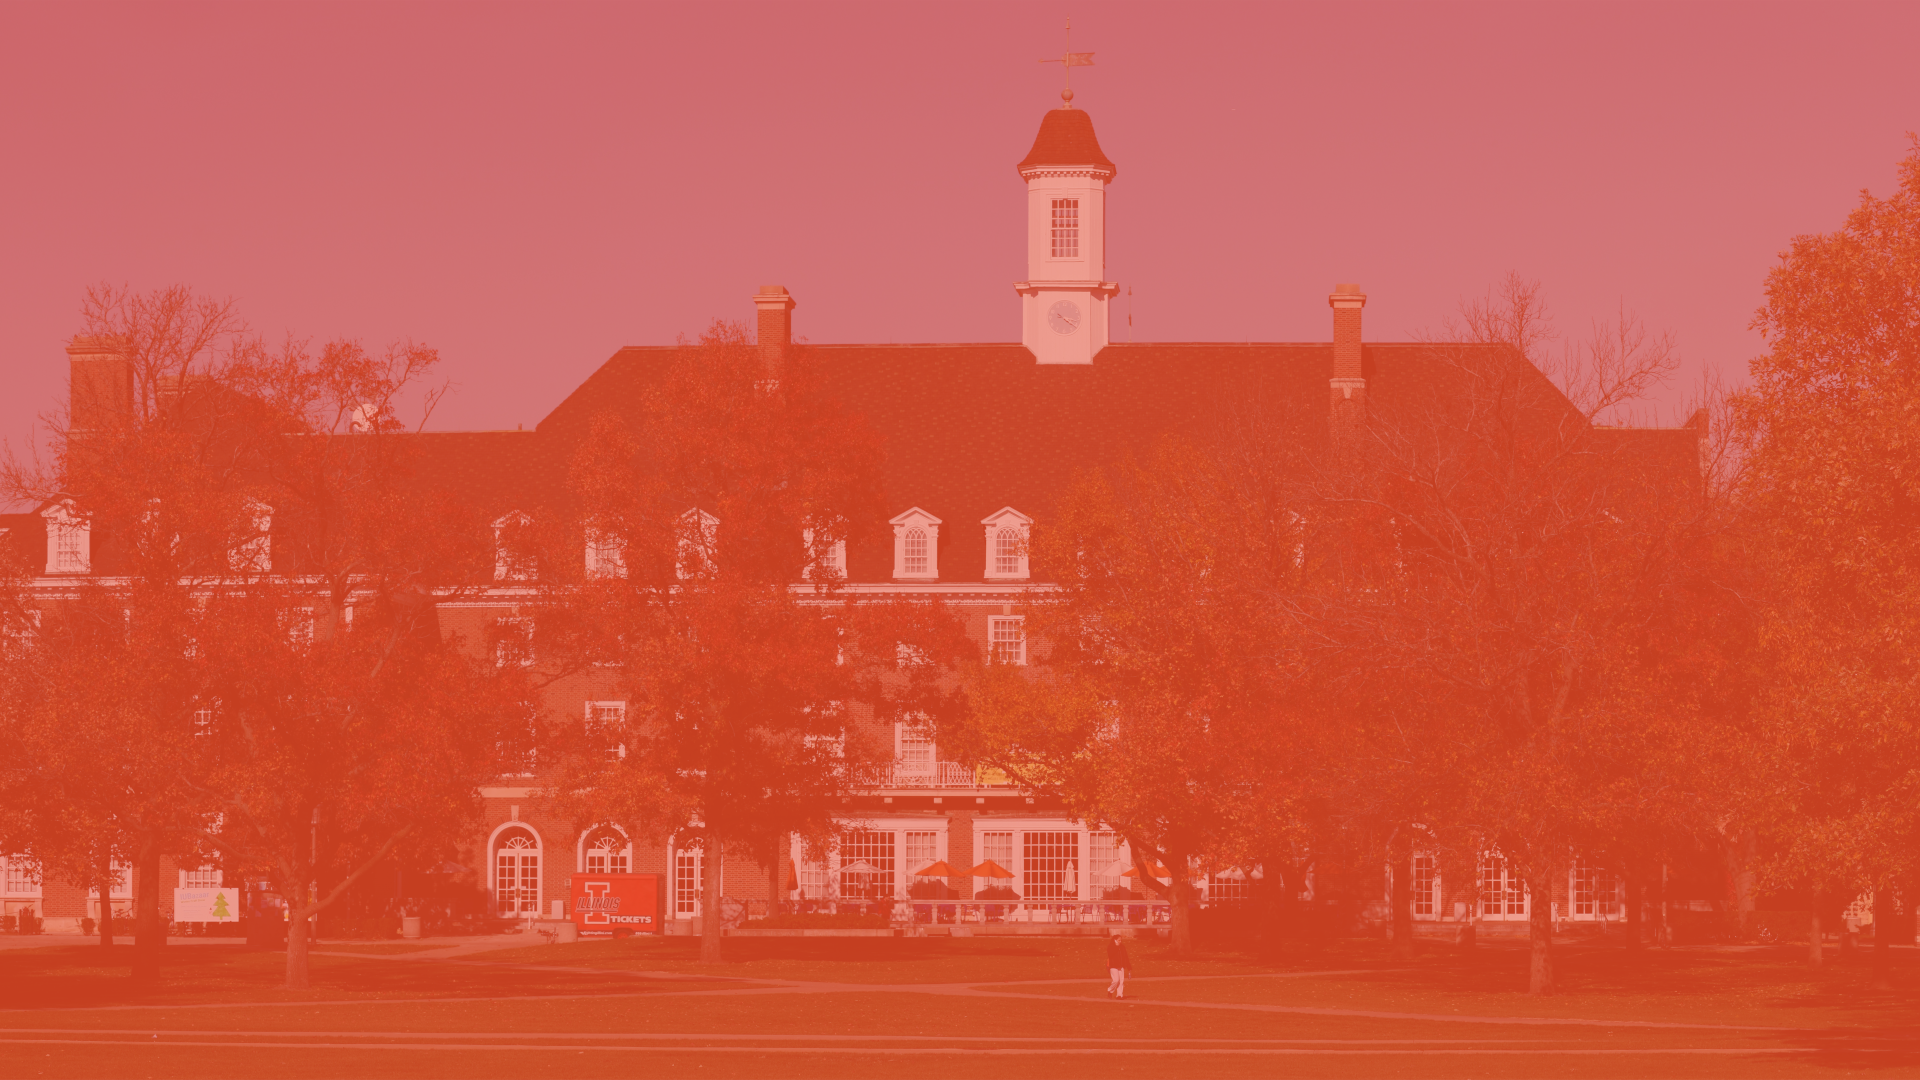
\includegraphics[width=\paperwidth, height=\paperheight]{imgs/uiuc.png}
    \end{textblock*} 
}{}

\begin{document}

\frame{\titlepage}

\section{Topics to Review}

\section{input and print}
\begin{frame}
  \frametitle{Input and Print}
  \begin{itemize}
    \item \underline{\textbf{The Input Function}}: A builtin function that gets a string from the user.
      \pause
      \begin{itemize}
        \item \textbf{input()} \textrightarrow Doesn't give a prompt.
          \pause
        \item \textbf{input(`A test input: ')} \textrightarrow Will output the message \textit{"A test input:"} to the screen and let the user type their input in after it.
          \pause
      \end{itemize}
    \item \underline{\textbf{The Print Function}}: A builtin function that takes a string as a parameter (in between the parentheses) and outputs that string
      \pause
      \begin{itemize}
        \item \textbf{print(`Hello, World!')} \textrightarrow Will output the `Hello, World!\n''. 
        \item \textbf{print(`Hello, World!', end="")} \textrightarrow Will output the `Hello, World!''. 
      \end{itemize}
  \end{itemize}
\end{frame}

\section{Data Types and Functions}


%
% Slide 9
%
\begin{frame}[fragile]
  \frametitle{Order and Mutability}
  % Please add the following required packages to your document preamble:
  \begin{table}[]
    \begin{tabular}{l|l|l}
      \hline
      \multicolumn{1}{c|}{}       & \multicolumn{1}{c|}{Ordered}                  & \multicolumn{1}{c}{Mutable}                  \\ \hline
      \multicolumn{1}{c|}{String} & \multicolumn{1}{c|}{\cellcolor[HTML]{34FF34}} & \multicolumn{1}{c}{\cellcolor[HTML]{FE0000}} \\ \hline
      List                        & \cellcolor[HTML]{34FF34}                      & \cellcolor[HTML]{34FF34}                     \\ \hline
      Tuple                       & \cellcolor[HTML]{34FF34}                      & \cellcolor[HTML]{FE0000}                     \\ \hline
      Set                         & \cellcolor[HTML]{FE0000}                      & \cellcolor[HTML]{34FF34}                     \\ \hline
      Dict                        & \cellcolor[HTML]{FE0000}                      & \cellcolor[HTML]{34FF34}                     \\ \hline
    \end{tabular}
  \end{table}
  \pause
  \begin{itemize}
      \pause
      \item This is a lot to remember. So memorize it through practice rather than through standard memorization. 
      \pause
      \item Remember to use the \lstinline|help()| function to lookup the list of functions you can use with each data types.
      \pause
      \item Python documentation.
      \pause
      \item \textbf{Test your code before submitting a resposne!}
  \end{itemize}
\end{frame}


\section{HTML}
%
% Slides
%
\begin{frame}[fragile]
    \frametitle{The Starting Template}
    \begin{lstlisting}[language=html,autogobble]
    <!DOCTYPE html>
    <html>
        <body>
            <h1>This is the header!</h1>
            <p> And this is my first paragraph :D </p>
        </body>
    </html>
    \end{lstlisting} 
    \vfill
    \begin{enumerate}
        \item \lstinline|<!DOCTYPE html>| \textrightarrow This defines the type of document we are making (html5) so the browser knows how to interpret it.
        \item \lstinline|<html>| \textrightarrow Defines the bounds of the HTML document.
        \item \lstinline|<body>| \textrightarrow Defines the visible portion of the html document.
        \item Headers:
            \begin{itemize}
                \item \lstinline|<h1>| \textrightarrow Largest header
                \item \lstinline|<h2>| \textrightarrow Second largest header
                \item \lstinline|<h3>| \textrightarrow You get the idea...
            \end{itemize}
        \item \lstinline|<p>| \textrightarrow Encapsulates a paragraph and formats the text as just plain text
    \end{enumerate}
\end{frame}

\section{requests}
\begin{frame}[fragile]
    \frametitle{Basics of Requests}
    \begin{enumerate}[A]
        \item Know how to make a get request and store a response object: \lstinline|r = requests.get(url)|
        \item Know the following main fields:
            \begin{itemize}
                \item \lstinline|r.text|
                \item \lstinline|r.status_code|
                \item \lstinline|r.content_headers|
            \end{itemize}
        \item Know basic status codes: 404, 200, 404, 502
    \end{enumerate}
\end{frame}

\section{General Review}
\begin{frame}[fragile]
    \frametitle{General Review Advice}
    \begin{enumerate}[A]
        \item The final will be much more representative of all topics.
        \item Be sure to review the review sheet. I make the review sheet as I make the tests so it's reflective of the content you can expect. 
        \item Be sure to practice testing your inputs during the practice exam.
    \end{enumerate}
\end{frame}


\end{document}
